\chapter{Introduction}
In the study of cosmology -- the process of understanding how the Universe came to be and what that Universe looks like today -- galaxies are perhaps one of the most important observational tracers, with which we can map and measure the makeup and structure of our Universe throughout cosmic time. As a result, robust models for the formation and evolution of galaxies are an essential aspect of the framework by which we might build a good understanding of our Universe. These collections of gas, stars and ambiguous dark matter are the direct result of the complex interplay between cosmology, gravitation and electromagnetic interactions that define the Universe which we live in, and so their characteristics are immutably tied to the very nature of our existence.

Of all the galaxies in our Universe, the one to which we have the closest access to understand the nuanced aspects of its formation and evolution is the galaxy within which we reside: the Milky Way -- \emph{the} Galaxy. The Milky Way presents the problem of galaxy formation at high fidelity, allowing us to test models for its genesis and evolution on a star-by-star basis. The assumption that our Galaxy is typical for its mass and other characteristics then allows us to extrapolate these models, trained on the Milky Way, to our understanding of galaxy evolution in general. The overarching goal of this thesis is to test that assumption, asking the question: \emph{is the Milky Way typical?}

By asking this question, we gain a means of properly calibrating any extrapolation of galaxy formation models, and will likely elucidate new aspects of the formation and history of the Milky Way through answering it. If the Milky Way \emph{is} a typical spiral galaxy, whose history is representative of the majority of galaxies at its mass and morphology, then it is a robust frame on which to develop models. If, however, the Milky Way is somehow \emph{atypical}, for example in its size, assembly history, stellar populations, dark matter content, or any other characteristic --  or combination of the above -- then it is important that the use of our detailed knowledge of the Milky Way should be tempered somehow to allow for these `atypicalities'. Of course, a detailed knowledge of the Milky Way only strengthens our understanding of its individual history of formation and assembly.

The means to answer the overarching question of the typicality of the Galaxy can only be established through a detailed understanding the place of our Galaxy in the Universe and its galaxy population. In this thesis we intend to make progress towards such an understanding by:
\begin{itemize}
    \item Developing a detailed and state-of-the-art picture of the present day structure and state of the Milky Way, to act as a stringent constraint on present and future models for its formation.
    \item Understanding how galaxies with similar characteristics to the Milky Way emerged, and how these galaxies compare to the mean galaxy population, through analysis of numerical simulations that accurately reproduce the broad properties of the galaxy population.
    \item Testing the predictions of cosmological simulations by reconstructing aspects of the assembly history of the Galaxy, using the most up-to-date data on the Milky Way.
\end{itemize}
The achievement of these more concentrated goals will allow for a re-assessment of the typicality of the Galaxy, and will inform the future interpretation of models for the formation and evolution of the Milky Way in the context of external galaxies.

\section{Galaxies in the cosmological context}

Before considering the state of our knowledge of the formation and evolution of the Milky Way, it is essential to set the scene of our current understanding of galaxies in general, and the connection of that understanding to the nature of the Universe. To this end, I briefly touch upon here some important aspects of galaxy formation theory in the cosmological context, with the aim of placing studies of the Milky Way into their much wider context.

\subsection{Galactic genesis}

In the current popular interpretation of modern cosmology, the cold dark matter model \citep[CDM, e.g.][]{1978MNRAS.183..341W}, galaxies are the eventual products of small scale fluctuations in the density field of the very early Universe, imprinted upon it by a rapid period of `inflation' very shortly after the Big Bang \citep{guth1981inflationary}. These `seed' fluctuations then collapsed under their own gravity as they became significant over the background density, which decreased with the expansion of the Universe. Dark matter, thought to interact with baryonic matter only through gravitation, filled these overdensities first, as it was not supported by the radiation which bakes the early Universe. As the density fluctuations grew with infalling dark matter, the baryonic matter slowly began to cool and collapse into the overdensities, forming the filamentary structure referred to as the `cosmic web'. The gas eventually collapsed deep into the potential wells of the dark matter, forming galaxies of great morphological variety - one of which became \emph{the} Galaxy: the Milky Way.

This simplified picture of structure formation followed by the genesis of galaxies demonstrates how the galaxy population of the Universe is the (indirect) result of cosmology. Na\"ively then, it seems like one could `reverse engineer' the galaxy population, and say something about the nature of our Universe, and in some sense, this is the overarching goal of studies of galaxy formation and evolution. However, this ideal is somewhat complicated by the non-linearity of the processes on galactic scales. The non-linearity of collapse and hierarchical build up of galaxies following the growth of the initial density fluctuations can only be properly realised through direct numerical simulation \citep[e.g.][]{2005Natur.435..629S}. I will argue in the course of this thesis that such simulations, which simulate the above processes self-consistently, and accurately model the hydro-dynamical processes that shape galaxies, are perhaps the most robust means of predicting the context of our Galaxy within CDM and other models.

\subsection{The galaxy-halo connection}
\label{sec:galaxyhaloconnect}
The study of the galaxy population has a long and colourful history. Of the many early realisations of the variety among galaxies in the Universe, and the perhaps more fundamental realisation of galaxies as external entities to the Milky Way, that which has perhaps best survived to present-day reference is the early work of \citet{1926ApJ....64..321H}, culminating in the widely known Hubble `Tuning-fork' diagram \citep[e.g.][]{1936rene.book.....H,1961hag..book.....S}. This diagram represents a useful summary of galaxy morphologies, but falls short of expressing the true variety of galaxies in our Universe, which display a broad spectrum of features such as bars, bulges, disks, rings, spirals, clumps, flocullence, fountains, streams and shells; all of which are the result of the myriad of processes that shape the galaxy population. Galactic (lower-case and capital G) astrophysics attempts to eke out the physics behind these structures and their connection to galaxy evolution theory and thus to cosmology and constraints on the currently accepted cosmological models. 

While direct constraints on the separate physical origins of all the features of the galaxy population are clearly out of easy reach, `broad-brush' approaches, such as correlating certain properties of galaxies with one another, lend some insight into the problem of galaxy evolution. For example, it is well established that galaxy morphologies correlate with their colours \citep[e.g.][]{2001AJ....122.1861S}, where blue (likely star-forming) galaxies tend to be those dominated by spiral and disk structures, and red (and therefore presumably non-star forming) galaxies are generally spheroidal in morphology. However, the Galaxy Zoo project \citep{2008MNRAS.389.1179L,2011MNRAS.410..166L}, which allowed for robust, citizen science driven, visual classification of an unprecedented sample of galaxies has shown that there are notable exceptions to this general trend \citep[ e.g.][]{2009MNRAS.396..818S,2010MNRAS.405..783M}. Furthermore, galaxies mainly fall into either of these camps, and very few reside in the intermediate `green' valley; galaxy colours are roughly bimodal \citep[e.g.][]{2004ApJ...600..681B,2006MNRAS.373..469B}. Such a colour bimodality suggests that if transitions between these groups occur, they occur very quickly. \citet{2006MNRAS.373..469B} showed that the fraction of galaxies in each group changes as a function of the number of a galaxy's projected neighbours, suggesting environment somehow plays a role in quenching star formation in the red, dead galaxies. \citet{2010ApJ...721..193P} separated the effects of environment and galaxy mass, demonstrating that star formation quenching is driven by both of these factors separately at different rates, where the environment tends to drive quenching mainly in satellite galaxies, and appeared to be independent of the mass of the haloes in which they reside \citep{2012ApJ...757....4P}. \citet{2013MNRAS.428.3306W} demonstrated that distance from the cluster center is a clearer defining factor of satellite quenching, and were able to reconcile the data with a dependence on halo mass. Quenching which is dependent on halo mass can be neatly framed as resulting from virial shock heating in the most massive haloes, which shuts down accretion by bringing gas cooling timescales above the dynamical time of the haloes \citep[e.g.][]{2006MNRAS.368....2D,2015MNRAS.447..374G}. Therefore, it may be that through the connection between their halo mass and colour, the galaxies as they appear to us are in some way a product of cosmology, via its dictation of the formation of structure. These results build up to a useful statement on the driving forces behind galaxy evolution, but are only one component of a comprehensive picture of the physics that forms galaxies in the variety we see.

A good example of an agent of galaxy evolution that is seemingly not \emph{directly} driven by cosmology, but is extremely important in reproducing the smaller scale ($\lesssim 0.01$ Mpc) structure in the Universe, is the effect of feedback. Feedback in galaxy formation refers to the regulation of star formation, usually via the attenuation of gas inflow by some process. Generally, feedback is divided into that from stellar sources, such as energy input from supernovae (SNe) or stellar winds, or that from black holes in the central regions of galaxies, e.g. active galactic nuclei (AGN). Allowing gas to collapse into galaxies without feedback means star formation proceeds at rates far higher than that observed, and reach stellar masses tens of times greater than those seen today. However, the inclusion of even relatively simple models for stellar feedback in early simulations and semi-analytic models brings galaxy masses closer inline with observations at the low mass end  \citep[$M\lesssim 10^{12}\ \mathrm{M_\odot}$ e.g.][]{1996ApJS..105...19K,1999MNRAS.310.1087S,2003MNRAS.339..312S}, whereas AGN feedback is necessary to suppress star formation in more massive galaxies \citep[$M\gtrsim 10^{12}\ \mathrm{M_\odot}$][]{2006MNRAS.370..645B,2008MNRAS.391..481S}, where energy injection from SNe is insufficient to pause cold flows. As a result of these feedback processes on both ends of the halo mass scale, the efficiency of star formation peaks in haloes of mass $\sim 10^{12}\ \mathrm{M_\odot}$ \citep[e.g.][]{2013ApJ...770...57B}, which as we will discuss later, is roughly the halo mass of the Milky Way. 

Not only is feedback thought to be important for the regulation of galaxy stellar masses, but likely also plays some role in eventual galaxy morphologies, in particular that of disk galaxies. Without sufficient feedback, low angular momentum material is not removed from central regions of simulated galaxies, which then do not reproduce properties of observed disks \citep[e.g.][and references therein]{2010MNRAS.408..812S}. However, including models for feedback that can efficiently eject such material to be re-accreted at later times with a higher angular momentum produces far more realistic disks, simulated self consistently in a cosmological context \citep[e.g.][]{2011MNRAS.415.1051B,2012MNRAS.427..379M,2013MNRAS.428..129S}. Therefore, the disk morphology of galaxies like the Milky Way is likely folded directly in with its history of feedback. Of course, stellar feedback is a direct result of the star formation history in any galaxy, which is dictated by the supply of gas at a given time, as we have discussed. If, as we touched on above, the gas supply to haloes hosting galaxies is dictated by their mass (to first order), then we arrive back at the large scale structure of the Universe and its cosmology. It is clear then that understanding the star formation and assembly of disk galaxies in detail, and the link to that offered by studying their morphology and stellar content, may provide important insights and constraints on models at even cosmological scales.


\section{The Milky Way as a disk galaxy}

% Having established the place of disk galaxies in our efforts to understand the Universe, and the importance of a detailed understanding of their formation and evolution, I now move to focus solely on that aspect of galactic astrophysics. I will summarise the current understanding of the Milky Way as a disk galaxy, before briefly describing the established model of galactic disk formation. In particular, I aim to introduce the extensive literature on the Milky Way from the last century, and explore the origin and development of near-field cosmology and Galactic archaeology -- the study of the Milky Way as a fossil remnant of the process of galactic formation and evolution (perhaps more accurately expressed as Galactic paleontology!).

Having established the importance of understanding the formation and evolution of disk galaxies in our efforts to understand the Universe, I now move to focus solely on this aspect of galactic astrophysics. Before discussing the progress thus far in understanding the history of formation and evolution of the Milky Way and other disk galaxies, I will first summarise what we know about the Milky Way as a galaxy. 

That we reside in a disk of stars was first postulated by the philosopher Immanuel Kant in 1755, shortly before William Herschel first mapped the shape of the Milky Way through star counting in 1785 \citep{Herschel01011785}. The fact that our Galaxy is just one of the many galaxies in the Universe was not properly understood until the early 20\textsuperscript{th} century, with the work of \citet{1929ApJ....69..103H}. Since that early work, we have come to be able to properly characterise our Galaxy and compare it to the others we observe, although as we will discuss, much of this knowledge is now being tested when confronted with the latest data.

The most obvious way by which to compare the Milky Way to its extra-galactic counterparts is through its morphology and structural parameters relating to its size. Such properties are readily measured for external galaxies and have been for some time \citep[e.g.][]{1959HDP....53..311D}. In terms of morphology, it is well established that the Milky Way has an extended stellar disk with spiral arms, a bulge component, a bar and a diffuse stellar halo with evidence of substructure. However, the exact details of these features are difficult to discern owing to the fact that much of the Galaxy is obscured by extinction as a result of our position in the disk. In this overview I will also discuss the connections between morphological components and trends in element abundances, with a view to later bringing these connections to bear on models for the formation of the Galaxy.

\subsection{The Disk}

The disk is the component of the Galaxy which we have arguably the best hope of understanding given the ease of access to its stars, at least in the Solar vicinity. The disk forms the main focus of this thesis, as it is the main component for which the data that are available from large Galactic surveys, pertain. Therefore, I will introduce the disk at a greater level of detail than the other components. This does not, however, mean that the disk is necessarily the part of the Galaxy with which we can attain the best understanding of its formation and evolution -- although, as I will discuss here, there are unexplained features of our disk for which a detailed understanding would provide a number of important constraints on the history of our Galaxy. 

\subsubsection{Spiral Structure}
The feature of our galaxy which can be compared to other disks with almost complete ubiquity is its spiral structure. However, our knowledge of the spiral structure is rather contentious. Mapping of the spiral structure is commonly performed in the near infra-red (NIR) and radio regime, overcoming much of the extinction to look at star forming regions of the Galaxy. Early studies of HII regions defined the `standard model' for the spiral structure of our Galaxy as a four armed spiral close to an Sc type with a $12^{\circ}$ pitch angle  \citep{1976A&A....49...57G}. More recent studies have have struggled to agree on the number of arms between 2 and 4 \citep[e.g.][]{1976A&A....46..261S,1980ApJ...239L..53C,1981ApJ...250..551B,1995ApJ...454..119V,2000A&A...358L..13D,2003A&A...397..133R}, generally because of the difficulties in measuring distances. Very Long Baseline Interferometry (VLBI) meaurements, which allow direct and precise trigonometric parallax and proper motion measurements favour a four armed spiral structure \citep{2009ApJ...700..137R,2014ApJ...783..130R}.

The nature of the spiral arms is the subject of much debate, splitting into two main streams between long lived stationary density wave models \citep[e.g.][]{1964ApJ...140..646L,1996ssgd.book.....B}, and models where the arms are transient and recurrent through the history of the disk \citep[e.g.][]{1981seng.proc..111T,1984ApJ...282...61S}. It is well established that tidal forces from satellites can give rise to transient spirals \citep[e.g.][]{2010MNRAS.403..625D}, but spiral patterns do arise in isolated simulations of thin disks. Indeed, the lifetime of the arms appears to be one of the more important questions to ask, which would discrimate between these models \citep{2011MNRAS.410.1637S}. In a recent example of how such a discrimination might be made, \citet{2018MNRAS.481.3794H} modelled the velocity field in the solar neighbourhood under the effects of transient winding spiral arm perturbations and found good agreement with \emph{Gaia} DR2 data. 

\subsubsection{Size and Thickness}
\label{sec:disksize}
The vertical extent of the disk is relatively well characterised at the solar radius due to the relative lack of extinction at high Galactic latititudes. For a long time, the disk has been divided into a thick and thin component, owing to the early results of \citet{1983MNRAS.202.1025G}, and the knowledge that such structures appear to exist in external disk galaxies \citep[e.g.][]{1979ApJ...234..829B,1979ApJ...234..842T,2006AJ....131..226Y}. Of many different measurements, a good baseline for the characteristic heights of these disk components is found in the tomography of M dwarfs from SDSS data in \citet{2008ApJ...673..864J}, who find exponential scale heights of 300 and 900 pc for the thin and thick component, respectively. In this sense, the Milky Way sits relatively well with external galaxy measurements, which have similar heights and also have radially extended thick components \citep[e.g][]{2006AJ....131..226Y}. However, the simple view of these disk components as geometric entities breaks down somewhat when the disk is dissected further.

A more natural separation can be made in the disk in its $\alpha$ element abundances (which we discuss further in Section \ref{sec:alpha}), whereby the disk can be divided into a high and low \afe{} component \citep[e.g.][]{1998A&A...338..161F,2003A&A...410..527B,2005A&A...433..185B,2013A&A...560A.109H,2014A&A...562A..71B,2014A&A...564A.115A,2014ApJ...796...38N,2015ApJ...808..132H}. These components are found to have similarities to the geometrically divided thin/thick disk, such that the high \afe{} disk has scale height $\sim 1$ kpc, and the low \afe{} disk has a scale height as low as $\sim 0.2$ kpc \citep[e.g.][]{2012ApJ...753..148B,2016ApJ...823...30B}. However, when defined in this way, the high \afe{} component has a relatively short scale length at $\sim 2$ kpc, compared to the geometrically defined thick disk which has a scale length closer to $\sim4$ kpc \citep{2008ApJ...673..864J}. The low \afe{} component has a flatter radial profile \citep{2012ApJ...752...51C}, which has a complex density structure resembling donut shaped annuli, such that the density increases out to a break radius, and decreases outside this radius \citep{2012ApJ...753..148B,2016ApJ...823...30B}. Furthermore, when the disk is divided into sub-populations according to the \afe{} and \feh{} abundances of its stars, it seems that the vertical mass distribution is smooth, suggesting that the `thick' disk may not be so distinct \citep{2012ApJ...751..131B}. Combining all the sup-populations, this can be reconciled with the double exponential found in the star counts by \citet{1983MNRAS.202.1025G} \citep[see][]{2013A&ARv..21...61R}. The vertical kinematics of the disk as a function of \afe{} are consistent with a smooth vertical structure \citep{2012ApJ...755..115B}, and it is clear that the high \afe{} disk is more kinematically hot than the low \afe{} stars \citep[e.g.][]{2005A&A...433..185B}. It is clear, therefore, that the link between the disk structure and its element abundances may be able to offer significant insight into the formation of the galaxy.

\subsubsection{Element Abundances}
\label{sec:diskabundances}
The disentangling of the origins of element abundance patterns in the solar vicinity and beyond offers many constraints on models for the formation of the Galaxy and it's star formation history \citep[a seminal review on the goals of this effort is given by][]{2002ARA&A..40..487F}. A good first order tracer of the history of star formation in the Galactic disk is offered by the metallicity of stars, as measured by their \feh{} abundance. \feh{}, as the primary ejecta of Type Ia supernovae (SNe), is a good indicator of the advancement of star formation in stellar populations. However, as I will discuss, the ratio of Iron abundance to that of the $\alpha$-elements, \afe{}, is a potentially more constraining diagnostic of the history of star formation in the disk. The many other element abundances which can be measured that originate from various sources are of course of great importance in understanding the history of the Milky Way, but I do not focus on these here.

Most models try and predict metallicity gradients in the disk and how these evolve over time. Metallicity gradients are measured by a variety of tracers by which the variation in the gradient with age can also be measured, including planetary nebulae \citep[e.g.][]{1994A&A...282..436M,1994Ap&SS.219..231M,2010ApJ...714.1096S,2011ApJ...738...27B}, open clusters \citep[e.g.][]{1998MNRAS.296.1045C,2002AJ....124.2693F,2004A&A...414..163S,2009A&A...494...95M,2016AN....337..922C} and field stars \citep[e.g][]{2004A&A...418..989N,2014A&A...566A..37G}. Among these studies, the trends between the \feh{} gradient and the tracer age seem to vary. This discrepancy was recently studied by \citep{2016arXiv160804951A} who, using precise age estimates in field stars, showed that the youngest stars have a gradient $d\mathrm{[Fe/H]}/dR = -0.058\pm 0.01\ \mathrm{dex\ kpc^{-1}}$, in agreement with measurements from Cepheid variables \citep{2014A&A...566A..37G}. In addition, they showed that older stars tend to have gradients closer to $\sim -0.07\ \mathrm{dex\ kpc^{-1}}$. By comparison of their data with numerical simulations, they showed that strong radial migration (which we discuss further in Section \ref{sec:galacticarchaeology}) and age systematics may account for some of the discrepanices.

By studying stellar metallicity distribution functions (MDFs) in the disk, even further insight can be gained on the history of the stellar disk. The MDF in the vicinity of the Sun is well characterised, and is roughly Gaussian with a mean \feh{} slightly less than solar at $\sim -0.1$ dex, and a standard deviation $\sim 0.2$ dex  \citep{1962AJ.....67..486V,2004A&A...418..989N,2011A&A...530A.138C,2012ApJ...761..160S}. For a long time, models which assumed no flow of gas in or out of the solar neighbourhood (closed-box models) over-predicted the number of metal poor stars \citep[the G-dwarf problem, e.g.][]{1963ApJ...137..758S,1975MNRAS.172...13P}. Uncovering the solution to this problem motivated the development of more detailed models which included prescriptions for the gas dynamics \citep[e.g.][]{1972Natur.236...21L,1976MNRAS.176...31L,1977ApJ...216..548T,1980FCPh....5..287T,1989MNRAS.239..885M}. The recent advent of large spectroscopic surveys that reach into the depths of the disk have lead to the characterisation of the MDF as a function of radius in the disk \citep[e.g.][]{2014A&A...564A.115A,2015ApJ...808..132H}, demonstrating that the MDF outside the solar radius diverges from Gaussian, showing a skew toward positive (negative) \feh{} in the outer (inner) disk. The explanation of this effect likely lies with radial migration of stars as shown in toy-models \citep{2015ApJ...808..132H} and using N-body simulations \citep{2016ApJ...818L...6L}.

While the metallicity, indicated by the Iron abundance, \feh{}, of stars gives a good first-order indication of the advancement of star formation, without studying the variation in the abundances of elements from different sources, it is difficult to build a complete picture of the history of star formation. As expressed above, Iron is the primarily ejected element in Type Ia SNe, but is also ejected in the SNe which occur in massive stars ($\gtrsim \ \mathrm{M_{\odot}}$), Type II SNe. However, Type II SNe also eject large amounts of elements which are produced through the fusion of $\alpha$ particles in the star before the explosion, and which are only ejected in trace amounts by Type Ia SNe - Oxygen, Neon, Magnesium, Silicon and Sulphur. This fact can be exploited to gain insights into the intensity of star formation in the Galaxy when stars were born. Because the progenitors of Type Ia SNe are white dwarf stars, which are only present in evolved stellar populations, these SNe have a characteristic delay time distribution (DTD), which is modelled based on observations as a power law, with a characteristic timescale of $\sim 1$ Gyr \citep[e.g.][]{2012MNRAS.426.3282M,2014ApJ...783...28G}. Conversely, Type II SNe begin exploding as soon as stars begin to form, as the lifetimes of massive stars are exceedingly short relative to the Type Ia timescale. While Type II SNe are exploding with little input from SNe Ia, the ISM becomes greatly enriched in $\alpha$ elements relative to Iron, and the \afe{} ratio is increased. If stars form in this enriched ISM before SNe Ia begin to dominate (i.e. if star formation is very intense), then the stellar population retains this \afe{} ratio. As SNe Ia turn on and begin to pollute the ISM with Iron (and little $\alpha$), the \afe{} of the ISM decreases. As the pollution of the ISM and re-ejection of polluted material from both types of SN proceeds, the \feh{} of formed stars gradually rises. This process produces a characteristic pattern in the stars populating the \feh{}-\afe{} plane, set by the intensity and timescale of star formation.

Such a pattern in \feh{}-\afe{} space is clearly visible in the solar vicinity, as shown in Figure \ref{fig:afe_split}. This Figure shows the \afe{} and \feh{} abundances for stars within 1 kpc of the sun, measured in the fourteenth data release (DR14) of the APOGEE survey (which is described fully in Section \ref{sec:APOGEE}). A divide between stars with enhanced \afe{} ratios, and those with roughly solar ratios is immediately obvious, and is indicated in the plot by the dashed line, representing visually determined split. In the high \afe{} stars, it is possible to make out a trend in \afe{} that is roughly flat below \feh{}$\sim -0.5$ dex, and then turns over and declines after that, joining the low \afe{} population. A trend between \afe{} and \feh{} is also visible in the low \afe{} stars after \feh{}$\sim -0.5$ dex, albeit with a shallower slope. The different trends between these abundance ratios is indicative that there may be some interesting feature in the history of the Galaxy that they arose from.

\begin{figure}
    \centering
    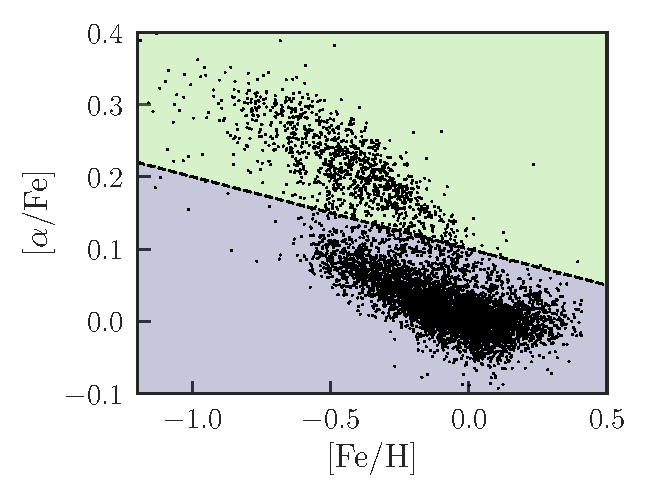
\includegraphics[width=0.8\textwidth]{thesis/Plots/afe_split_colors.pdf}
    \caption[The \feh{} and \afe{} abundances of stars in the solar vicinity from APOGEE DR14, indicating the bimodality in \afe{} at fixed \feh{}]{The \feh{}-\afe{} plane for stars located near the Sun (within 1 kpc) from the fourteenth data release (DR14 of the APOGEE survey). The coloured regions indicate a rough selection of stars with high (\emph{green}) and low (\emph{blue}) \afe{}. A bimodality in \afe{} is clearly present, at fixed \feh{}, between $-0.5 \lesssim \mathrm{[Fe/H]} \lesssim 0.0$ dex. The two populations appear to overlap at roughly solar \feh{}.}
    \label{fig:afe_split}
\end{figure}

These populations have, of course, been studied extensively since their discovery \citep[e.g.][]{1998A&A...338..161F,2003A&A...410..527B,2005A&A...433..185B,2013A&A...560A.109H,2014A&A...562A..71B,2014A&A...564A.115A,2014ApJ...796...38N,2015ApJ...808..132H} and, as expressed in Section \ref{sec:disksize}, have important links to the spatial structure of the Galaxy. Along with the MDFs (mentioned above), large scale spectroscopic surveys have also unveiled the stellar \feh{}-\afe{} distribution over great extents of the disk.  \citet{2014ApJ...796...38N} demonstrated that the positions of Red Clump (RC) stars (whose distances can be accurately measured by the fact that they are standard candles) in \feh{}-\afe{} space change as a function of Galactocentric radius and height. \citet{2015ApJ...808..132H} followed up on that work by showing a similar trend in a much larger sample Red Giant Branch stars. The findings of both studies were that that the mean \feh{} of the low \afe{} stars appears to move to higher \feh{} at smaller $R$, while the high \afe{} stars dominate the distribution at high $z$, and occupy a similar locus everywhere in the disk but appear to decline in density with $R$. These results place very strong constraints on any model which hopes to explain the origin of these element abundance trends, and I will briefly discuss such models in Section \ref{sec:galacticarchaeology}.

\subsection{The Bulge and Bar}

I discuss the bulge of the Milky Way in coordination with the bar, as these components are co-spatial in the center of our Galaxy and have a history and origin which is likely linked in some way, at some point in time. While the bulge is harder to study given the increased effect of extinction and problems with contamination by disk stars in bulge fields, a number of landmark studies have been able to elucidate its structure and its connection to the origin of the central region of the Galaxy.

\subsubsection{\emph{Pseudo}-bulges, boxes and peanuts}
During the early years of studying the Milky Way bulge, there was much debate as to its origin. The main arguments were either that it built up in the early history of the Galaxy through the merging of its satellite galaxy progenitors -- and thus is a `classical' bulge, resembling the structure of elliptical galaxies, which are thought to be built by the same process -- or that it formed in a secular fashion from stars in the disk or bar of the galaxy to become a `pseudobulge' \citep[a useful summary of these definitions is provided in Section 1.1 of][]{2004ARA&A..42..603K}. There now exists a wealth of evidence to suggest that while external galaxies certainly do host classical bulges \citep[e.g.][]{2009MNRAS.393.1531G}, the Milky Way itself is more likely host to a bulge with a structure indicative of secular processes - a pseudobulge. The Galactic bulge is boxy in shape \citep[e.g][]{1995ApJ...445..716D}, and is proposed to be formed via the heating of stars by buckling of a bar which formed from the stellar disk \citep[e.g.][]{1981A&A....96..164C,1991Natur.352..411R}.

As mentioned above, it was the work of \citet{1995ApJ...445..716D}, exploiting COBE infra-red data who revealed what is now referred to as the Boxy/Peanut (B/P) morphology of the Milky Way bulge. Prior to this, in perhaps the first direct evidence for a bar in the Milky Way, \citet{1991ApJ...379..631B} had shown the presence of asymmetry in $2.4 \mu$m balloon observations \citep{1982AIPC...83...48M} toward the Galactic centre, consistent with predictions for a bar of \citet{1979A&AS...37..403S} and \citet{1980ApJ...236..779L}. This broad picture of a B/P bulge plus a bar has prevailed to the present day, although the exact nuances of its structure are still the subject of debate.

Red Clump (RC) stars have proved to be essential in studying the structure of the Bulge. Red Clump stars are helium burning, horizontal-branch stars whose luminosity is found to have very little dependence on both age and metallicty, and so make good standard candles. Observing RC stars along lines of sight to the bulge allows for the mapping of its structure. Upon observing bulge RC stars Multiple groups find that there exists a split in the Red Clump at latitudes $|b| > 5^{\circ}$, where each branch of the split represents an RC population at a different distance, at either side of an X-shaped structure \citep{2010ApJ...721L..28N,2010ApJ...724.1491M,2011AJ....142...76S}. Later, using RC giants in the VVV survey, \citet{2013MNRAS.435.1874W} performed a more complete measurement of the 3D bulge structure, confirming the X-shape seen in the older observations. Recently, \citet{2016AJ....152...14N} used WISE images to make a clear imaging of the X-shape. Such X-shaped structures appear in many external disk galaxies \citep[e.g.][]{2006MNRAS.370..753B}, and are thought to arise as a consequence of the instabilities in the disk which give rise to the B/P morphology \citep[based on studies of N-body simulations, e.g.][]{2005MNRAS.358.1477A,2006ApJ...645..209D}.

Aside from morphological constraints on the bulge and bar, much effort has been made to model the dynamical effects of this structure on stars at the solar radius. As an example, it is contended by various groups that the Hercules stream in the solar neighbourhood (of stars moving together with heliocentric velocity $U \sim -30\ \mathrm{km\ s^{-1}}$ and $V \sim -50\ \mathrm{km\ s^{-1}}$), is the result of a perturbation by the outer Lindblad resonance (OLR) of a short ($\sim 3$ kpc), fast bar \citep{2000AJ....119..800D,2014A&A...563A..60A,2017MNRAS.466L.113M}. However, other groups claim that a longer bar ($\sim 5$ kpc) is necessary to best fit star counts from a variety of surveys \citep{2015MNRAS.450.4050W}, suggesting a more slowly rotating bar with an OLR further out in the disk \citep[although see][for a reconciliation of Hercules with a long, slow bar]{2018MNRAS.477.3945H}. The connection between the bar and the local velocity distribution, and the current model of the disk origin for the Milky Way bulge are both suggestive of the importance of understanding the complexities of the interaction between the different components of the Galaxy.

\subsubsection{Element Abundances and the Age of the Bulge}
Where element abundances are considered, the central regions of the Galaxy bear some similarities to the disk, and some important differences. Early studies of abundances in the bulge relied on small samples in regions of low extinction \citep[e.g.][]{1994ApJS...91..749M}, revealing that stars in these regions had an intermediate metallicity (\feh{} $\sim -0.25$ dex), and were enhanced in Aluminium. The vertical gradient of \feh{} accross the bulge is negative, which was originally considered incompatible with a purely disk origin of this component, and suggesting that the Milky Way had at least some classical bulge component \citep[e.g.][]{2008A&A...486..177Z}, however the kinematics of the bulge place very low upper limits on the mass of this component \citep[e.g. $\sim 8\%$;][]{2010ApJ...720L..72S}. A closer look at the metallicity distribution in the bulge with better data from the ARGOS survey revealed that the bulge stars divide into sub-populations in \feh{} space, amounting to a wide MDF spanning a range $-2.8 \lesssim \mathrm{[Fe/H]}\lesssim 0.6$ dex \citep{2013MNRAS.430..836N}. The ARGOS data appear to be consistent with an entirely disk instability driven origin of the bulge.

Alternate element abundances which provide a way to test models for the bulge formation are $\alpha$-elements, which trace star formation as described in Section \ref{sec:diskabundances}. Many bulge stars have enhanced \afe{}, and appear similar in their \afe{} and \feh{} to local stars in the \afe{} enhanced disk \citep{2010A&A...513A..35A,2015A&A...584A..46G}, suggesting a similar timescale for star formation. However, by taking high resolution spectra of microlensed dwarfs in the bulge, \citet{2013A&A...549A.147B} found that the `knee' in the bulge \afe{}-\feh{} plane is at a slightly higher \feh{} than the local disk, suggesting a slightly faster enrichment history in the center of the galaxy. The \afe{}-\feh{} distribution as seen by APOGEE in different radius and height bins from the Galactic center to the solar vicinity \citep{2016PASA...33...22N} also seems to suggest that the high \afe{} stars in the solar vicinity are in some way connected to those in the central region of the galaxy.

In terms of actual stellar age, the bulge is generally considered to be built of relatively old stars, at least older than those in the disk. The mean age of the bulge which can be measured from the colour-magnitude diagrams of giant stars in the bulge obtained from deep photometry is $\sim 10$ Gyr \citep[e.g.][]{2003A&A...399..931Z,2013A&A...559A..98V}, and it seems that there are very few stars younger than $\sim 5$ Gyr\citep{2011ApJ...735...37C}. Measuring ages using colour-magnitude diagrams in the bulge is notoriously difficult owing to difficulties in subtracting foreground disk contaminants, and uncertainties in reddening estimates and (usually) unmodelled effects of the metallicity distribution, leading to uncertainties of the order of $\sim 2$ Gyr \citep{2016ASSL..418..199G}. A very old bulge is interpreted as being indicative of one built via merging processes (a classical bulge), given that disk instabilities should bring young stars into the bulge. The microlensed dwarf sample of \citet{2013A&A...549A.147B} suggests that there may indeed be a population of young stars in the bulge, finding that 22\% of the dwarfds were younger than 5 Gyr old. Therefore, it seems that finding accurate age estimation methods for giants in the bulge may be able to provide stronger constraints on the classical vs. pseudobulge problem.

\subsection{The Stellar Halo}
The halo of the Milky Way is the component which can be most readily observed without encountering many issues with extinction (at least above and below the plane of the disk). The halo undoubtedly can provide a wealth of information on the history of the galaxy, owing to the fact that dynamical timescales are much longer than in the disk or bulge, preserving dynamical traces of past merger events in coherent stellar debris referred to as streams \citep[e.g.][]{1996ApJ...465..278J}. The halo and the stellar substructure within it may be among the best means of measuring the mass and inferring the gravitational potential of the Milky Way halo \citep[e.g.][]{2014ApJ...794....4P}. For this reason, the detailed understanding of its structure and the origin of it is of great importance to developing a complete picture of the formation of the Galaxy. Here I will briefly touch upon some of the important features of the halo and how these connect to its overall evolution.

\subsubsection{Structure}
As mentioned above, the long dynamical timescale in the halo means that phase space sub-structures are likely not readily erased. A good example of such a structure is the Sagittarius dwarf galaxy, which has survived many orbits around the Galaxy \citep[e.g.][]{1997AJ....113..634I}, and whose stellar stream is mapped over $\sim 100$s of degrees \citep[e.g.][]{2003ApJ...596L.191N,2004AJ....128..245M,2006ApJ...642L.137B,2009ApJ...700.1282Y}. Sagittarius is just one of a panoply of known groups of accreted stellar material \citep[see e.g.][for a review]{2013NewAR..57..100B}, which indicate that at least some part of the stellar halo is built from the accretion of smaller systems \citep[as predicted in the seminal work of][which we discuss further in Section \ref{sec:galacticarchaeology}]{1978ApJ...225..357S}. These lumps in the density profile of the halo must be accounted for when measuring its overall structure \citep[e.g.][]{2011MNRAS.416.2903D}. The mass in stellar substructure in the halo must also be accounted for when estimating its total stellar mass, and is estimated to be of the order $10^8\ \mathrm{M_{\odot}}$ \citep[based on a recent review by][]{2016ARA&A..54..529B}. Once substructure is accounted for, then the stellar halo can be fit with a relatively smooth density model.

The density distribution of the smooth part of the halo is well characterised using a variety of tracers whose distances can be determined to a good level of accuracy, such as RR Lyrae stars 
\citep[e.g.][]{2009MNRAS.398.1757W,2010ApJ...708..717S,2013AJ....146...21S,2014ApJ...788..105F}, blue horizontal branch (BHB) and blue straggler stars \citep[e.g.][]{2011MNRAS.416.2903D}, main-sequence turn-off (MSTO) stars \citep[e.g.][]{2011ApJ...731....4S} and red giant branch (RGB) stars \citep[e.g.][]{2015ApJ...809..144X}; a good overview of the results from all of these studies can be found in \citet{2016ARA&A..54..529B}. The halo density profile is fit across all these studies by power-law, with an index $\sim-2.5$ in the inner parts. Additionally, most of the aforementioned works agree that the inner halo is flattened somewhat, by a factor somewhere in the region of $\sim 0.65$. It is also generally agreed, from the farthest reaching data, that the density profile steepens with radius with a break in the power-law at a break radius $r_{\mathrm{b}}\sim 25$ kpc. Such a break in the halo density profile is thought to be related to the accumulation of stars at the apocenter of a relatively massive accretion event(s) \citep{2013ApJ...763..113D}, and is not a ubiquitous feature of galaxy haloes \citep[a good example being the lack of such a break in M31, e.g.][]{2011ApJ...739...20C}.
\subsection{The Local Group}

\section{Unearthing fossilised galaxy formation in the Milky Way}
\label{sec:galacticarchaeology}
\subsection{A schematic for the formation of disk galaxies}

A useful way to present the wealth of work on the formation of the Milky Way is to describe a schematic of its formation as a disk galaxy, as unveiled by studies of it throughout the last century. The conception of the `canonical' model for the birth of the Milky Way in a rapid collapse of a proto-galactic gas cloud \citep[the ELS model;][]{1962ApJ...136..748E} makes a good starting point for such a schematic. 

In what can be considered as the first implementation of Galactic archaeology, \citet{1962ApJ...136..748E} showed that the orbital energies and eccentricities of stars with lower metallicities were increased, inferring that these stars were members of the first generation of stars formed from the originally rapidly collapsed protocloud of our galaxy. The later work of \citet{1978ApJ...225..357S}, which inferred that the varying element abundances of Galactic globular cluster (GC) systems, suggested a different view of the formation of the galaxy through the conglomeration of `protogalactic fragments'. These seminal works underpin many of the modern studies of the Milky Way, and are commonly framed as competitive scenarios. However, at the time, these findings mirrored the developments in the CDM model \citep{1978MNRAS.183..341W}, and analytical models of the collapse of gas in a halo which gained angular momentum from hierarchical clustering produced seemingly realistic disks \citep{1980MNRAS.193..189F}. While analytic approaches would work well at describing galaxy disk formation, hydrodynamical simulations in a cosmological context struggled to produce realistic populations of disk galaxies until advances in the inclusion of detailed feedback models, as expressed in Section \ref{sec:galaxyhaloconnect}. 



